\documentclass{TIJMUjiaoanLL}
\pagestyle{empty}

\begin{document}

\kecheng{分子生物计算}
\neirong{突变和随机化 \ / 第7章}
\jiaoshi{伊现富}
\zhicheng{讲师}
\riqi{2015年10月12/16/19日8:00-10:00}
\duixiang{生物医学工程与技术学院2013级生信班(本)}
\renshu{28}
\fangshi{理论讲授}
\xueshi{6}
\jiaocai{Perl语言在生物信息学中的应用——基础篇}

\firstHeader
\maketitle
\thispagestyle{empty}

\mudi{
\begin{itemize}
  \item 掌握:随机选取数组元素的方法;随机选取字符串位置的方法;随机选取两个整数间数字的方法。
  \item 熟悉:随机化在模拟DNA突变和生成随机DNA序列中的应用。
  \item 了解:随机数生成器及其种子。
  \item 自学:自上而下和自下而上的程序设计理念。
\end{itemize}
}

\fenpei{
\begin{itemize}
  \item (15')引言与导入:回顾突变的概念、原因和类型,介绍随机和模拟及其在DNA突变中的应用。
  \item (10')随机数生成器:介绍随机数生成器、伪随机数以及种子的相关概念。
  \item (75')随机化程序:通过生成随机句子的Perl程序讲解随机化在Perl语言中的实现。
  \item (50')模拟DNA突变:通过模拟DNA突变的Perl程序讲解随机化在模拟DNA突变中的应用。
  \item (50')生成随机DNA:通过生成随机DNA序列的Perl程序讲解随机化在生成随机DNA序列中的应用。
  \item (90')分析DNA:详细讲解如何基于已有的知识生成随机DNA序列并对它们进行相似性比较。
  \item (10')总结与答疑:总结授课内容中的知识点与技能,解答学生疑问。
\end{itemize}
}

\zhongdian{
\begin{itemize}
  \item 重点:随机选取数组元素;随机选取字符串位置;随机选取两个整数间的数字。
  \item 难点:随机选取数组元素;嵌套循环的工作步骤。
  \item 解决策略:通过实例演示帮助学生理解、记忆。
\end{itemize}
}

\waiyu{
\vspace*{-10pt}
\begin{multicols}{2}
突变(mutation)

随机性(randomness)

模拟(simulation)

随机数生成器(random number generator)

伪随机性(pseudorandomness)

种子(seed)

\end{multicols}
\vspace*{-10pt}
}

\fuzhu{
\begin{itemize}
  \item 多媒体:突变的类型;随机化在Perl语言中的实现。
  \item 板书:模拟DNA突变的步骤;嵌套循环的工作步骤。
  \item 演示:通过随机化模拟DNA突变、生成随机DNA序列。
\end{itemize}
}

\sikao{
\vspace*{-10pt}
\begin{multicols}{2}
\begin{itemize}
  \item 如何设置Perl语言随机数生成器的种子?
  \item 如何随机选取数组的元素?
  \item 如何随机选取字符串中的位置?
  \item 如何随机选取两个整数间的一个数字?
  \item 比较自上而下和自下而上的程序设计理念。
  \item 解释嵌套循环的工作步骤。
\end{itemize}
\end{multicols}
\vspace*{-10pt}
}

\cankao{
\begin{itemize}
  \item Beginning Perl for Bioinformatics, James Tisdall, O'Reilly Media, 2001.
  \item Perl语言入门(第六版),Randal L. Schwartz, brian d foy \& Tom Phoenix著,盛春\ 译,东南大学出版社,2012。
  \item Mastering Perl for Bioinformatics, James Tisdall, O'Reilly Media, 2003.
  \item 维基百科等网络资源。
\end{itemize}
}

\firstTail

\newpage
\otherHeader

\begin{enumerate}
  \item 引言与导入(15分钟)
    \begin{enumerate}
      \item 突变
	\begin{enumerate}
	  \item 简介
	    \begin{itemize}
\parpic[fr]{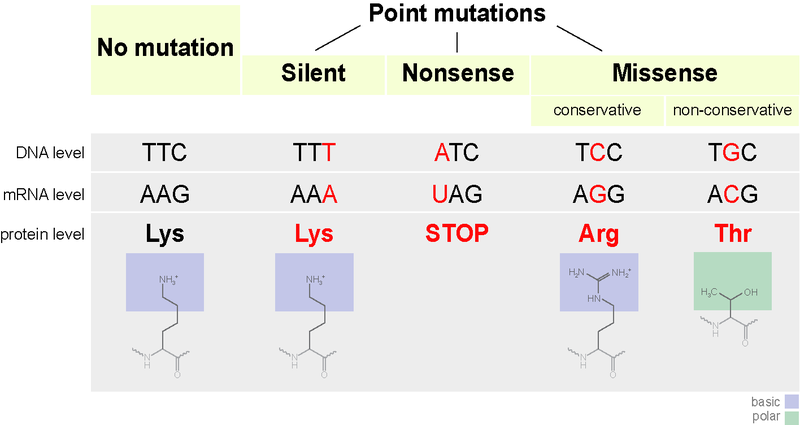
\includegraphics[width=0.45\textwidth]{c7.mutation.point.01.png}}
	      \item 定义:突变,即基因突变,指细胞中的遗传基因发生的改变
	      \item 原因:复制错误、化学毒性、物理辐射、生物病毒……
	      \item 影响:细胞死亡或者癌变;进化的“推动力”\textcolor{red}{(双刃剑!)}
	      \item 类型:点突变、插入、删除、重复、倒位、易位……
	    \end{itemize}
	  \item 点突变
	    \begin{itemize}
	      \item 简介:单一核苷酸替换成了另一核苷酸\textcolor{red}{(狭义 vs. 广义)}
	      \item 分类
		\begin{itemize}
		  \item 转换(嘌呤变嘌呤,嘧啶变嘧啶),颠换(嘌呤变嘧啶,嘧啶变嘌呤)
		  \item 同义突变(氨基酸产物不变),错义突变(氨基酸产物改变),无义突变(氨基酸变成终止密码)
		\end{itemize}
	    \end{itemize}
	\end{enumerate}
      \item 随机:一个不定因子不断产生的重复过程,可能遵循某个概率分布\textcolor{red}{(vs. 任意)};(进化论)随机突变
      \item 模拟:通过随机化模拟DNA突变
      \item 即将学习
	\begin{itemize}
	  \item 随机选取数组元素,随机选取字符串位置
	  \item 模拟DNA突变:随机选取DNA中的一个核苷酸突变成一个随机的核苷酸
	  \item 根据要求生成随机DNA序列数据集
	  \item 重复突变DNA来研究突变随时间累积的影响
	\end{itemize}
    \end{enumerate}
  \item 随机数生成器(10分钟)
    \begin{enumerate}
      \item 随机数生成器:通过一些算法、物理讯号、环境噪音等来产生看起来似乎没有关联性的数列的方法或装置\textcolor{red}{(丢硬币、掷骰子、洗牌)}
      \item 伪随机数:重复周期比较大的数列,并不是真正的随机数,按一定的算法和种子值生成
      \item 种子:种子改变,伪随机数随之改变;种子本身应该是随机选择的
    \end{enumerate}
  \item 随机化程序(75分钟)
    \begin{enumerate}
      \item Perl程序7.1:通过随机选取名词、动词和介词构造句子
      \item 设置随机数种子:\verb=srand(time | $$);=
	\begin{itemize}
	  \item time:时间;\verb|$$|:PID;\verb=|=:位或
	  \item \verb|srand;|会自动设置种子;rand会自动调用srand设置种子
	\end{itemize}
      \item \textcolor{red}{【重点、难点】}随机选取数组元素\textcolor{red}{(比较并理解三种不同的写法)}
	\begin{itemize}
	  \item \verb|$verbs[ int( rand( scalar @verbs ) ) ]|\textcolor{red}{(由内而外层层解析)}
	  \item \verb|$verbs[ int rand scalar @verbs ]|
	  \item \verb|$verbs[rand @verbs]|
	\end{itemize}
      \item \textcolor{red}{【重点、难点】}\verb|$verbs[rand @verbs]|
	\begin{itemize}
	  \item rand期望一个标量值,所以会把 \verb|@verbs|放在标量上下文中进行求值,返回数组元素个数
	  \item 数组的下标总是整数值,所以当它需要下标时,会自动提取小数的整数部分,因此不再需要int
	\end{itemize}
    \end{enumerate}

\otherTail
\newpage
\otherHeader

  \item 模拟DNA突变(50分钟)
    \begin{enumerate}
      \item \textcolor{red}{【重点】}编写子程序\textcolor{red}{(对每一个子程序都单独进行测试)}
	\begin{itemize}
	  \item 随机选取DNA序列中的一个位置\textcolor{red}{(借鉴随机选取数组元素的策略)}
	  \item 随机选取一个核苷酸\textcolor{red}{(每一个子程序都可能有改进的空间)}
	  \item 实现DNA序列上的一次突变\textcolor{red}{(充分利用已经编写完成的子程序)}
	\end{itemize}
      \item 组合子程序\textcolor{red}{(体会子程序的便利;总结分割子程序的经验)}
	\begin{itemize}
	  \item Perl程序7.2:组合需要的子程序模拟DNA突变
          \item 改进程序:保证突变成和原核苷酸不同的核苷酸
	\end{itemize}
      \item 声明变量
	\begin{itemize}
	  \item 在程序顶部统一声明 vs. 第一次使用时声明
	  \item 局部变量(在代码块中声明) vs. 全局变量(在主程序中声明)
	\end{itemize}
    \end{enumerate}
  \item 生成随机DNA(50分钟)
    \begin{enumerate}
      \item 设计理念\textcolor{red}{(理念不同,目的相同;比较并练习不同的设计理念)}
	\begin{itemize}
	  \item 自上而下:从主程序开始,当需要子程序再进行编写
	  \item 自下而上:从子程序开始,逐步组装出完整的主程序
	\end{itemize}
      \item 伪代码
	\begin{itemize}
	  \item 总体目标:生成一系列长短不一的随机DNA片段
	  \item 自上而下\textcolor{red}{(将大任务逐步分割成容易实现的小目标)}
	    \begin{enumerate}
	      \item 生成一系列长短不一的随机DNA片段
	      \item 编写 \verb|make_random_DNA_set|子程序
	      \item 编写 \verb|make_random_DNA|子程序
	      \item 编写 \verb|randomnucleotide|子程序
	    \end{enumerate}
	\end{itemize}
      \item Perl程序7.3:根据要求生成一系列长短不一的随机DNA片段
	\begin{itemize}
	  \item \textcolor{red}{【重点】}随机选取两个整数间的一个整数\textcolor{red}{(妙用rand函数;理解+1的原因)}
	    \begin{itemize}
	      \item \verb|int( rand( $maxlength - $minlength + 1 )  ) + $minlength|
	    \end{itemize}
	\end{itemize}
    \end{enumerate}
  \item 分析DNA(90分钟)
    \begin{enumerate}
\parpic[fr]{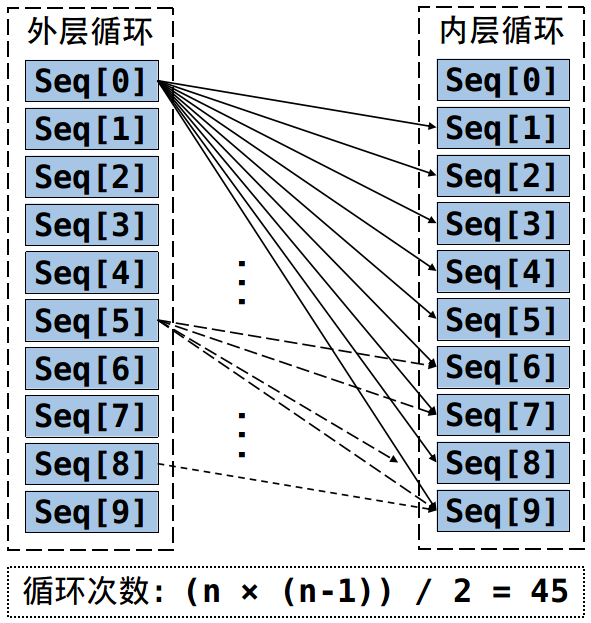
\includegraphics[width=0.45\textwidth]{c7.mutation.nested.loop.png}}
      \item 问题:两条DNA序列的相似性如何?
      \item Perl程序7.4:计算一个DNA数据集中两两之间相似性百分比的平均值
      \item \textcolor{red}{【难点】}嵌套循环\textcolor{red}{(注意内外两层循环初始值和终止值的差别)}
    \end{enumerate}
  \item 总结与答疑(10分钟)
    \begin{enumerate}
      \item 知识点
	\begin{itemize}
	  \item 随机:数组元素,字符串位置
	  \item 随机数生成器:伪随机,种子
	  \item 程序设计理念:自上而下,自下而上
	  \item Perl语言:变量声明,嵌套循环
	\end{itemize}
      \item 技能
	\begin{itemize}
	  \item 熟练使用Perl语言中的随机数生成器
	  \item 熟悉自上而下和自下而上的设计理念
	  \item 用Perl编写DNA突变相关的程序
	\end{itemize}
    \end{enumerate}
\end{enumerate}

\otherTail

%\parpic[fr]{\includegraphics[width=\textwidth]{}}

\end{document}
